\section{Propuesta 1}
\label{sec:propuesta_1}

    El sistema presenta una degradacion principalmente por el manejo indevido del log.
    Destacamos que la posibilidad de permitir consultar el log de manera completa es la principal causa de degradacion.
    Este escala con el numero de operacion, lo que provoca un aumento en el uso de recursos para mantenerlo, y un aumento en los tiempos de respuesta para consultarlo.
    Esto arrastra la degradacion a los otros endpoints, entre ellos exchange, el principalmente mencionado por los usuarios.

    Destacamos que un endpoint que permite consultarlo todo por definicion no es escalable, recomendamos la implementacion de paginacion.
    Sinembargo, asumimos que esta es un requerimiento de negocio y que las mejoras propuestas no deben alterar la firma del sistema para con los usuarios.
    Se propone desacoplar el log para que la degradacion de este no afecte a los endpoints de negocio del sistema.
    Proponemos agregar un nodo dedicado, analogo a exchange-api para el manejo del log.
    Algunas optimizaciones de la implementacion que consideramos que vale la pena mencionar son:

    \begin{itemize}
        \item Remplazamos el uso del formato .json para el almacenamiento a .ndjson, de esta manera podemos agregar los registros al final sin reescribir todo el archivo.
        \item El archivo ya no se carga en memoria, se stremea el cliente directamente desde disco en batches. Destacamos que agregamos los caracteres [ al inicio y ] al final del stream para mantener la firma original con respecto al formato .json.
        \item Solo enviamos hasta el ultimo byte valido disponible al momento de recibida la consulta y verificamos que la ultima entrada sea valida (evita race condition con la escritura).
        \item Exchange api loguea directamente al nuevo nodo dedicado mediante una conexion TCP dedicada.
    \end{itemize}

    \begin{figure}[H]
        \centering
        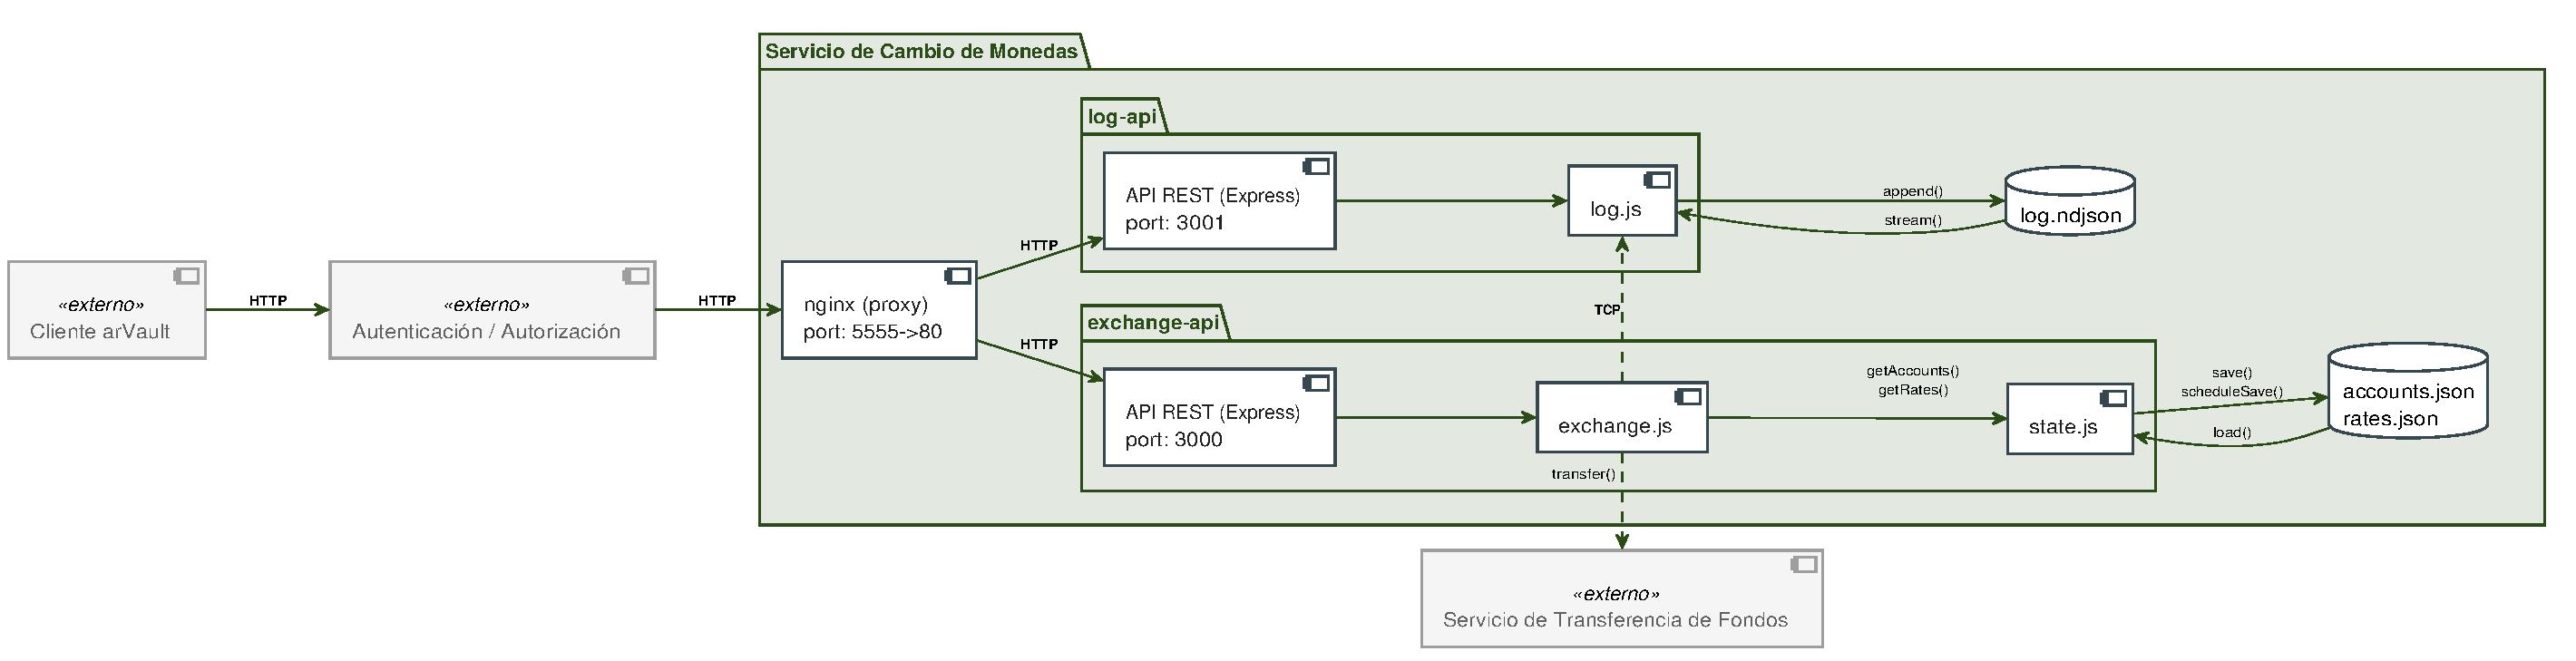
\includegraphics[width=1\columnwidth]{figures/diagramas/componentes_y_conectores_propuesta_1}
        \caption{ Diagrama Components \& Connectors de la propuesta 1. }
        \label{fig:propuesta_1_componentes_y_conectores}
    \end{figure}

    \subsection{Impacto en los QA}
    \label{sec:propuesta_1_impacto_en_los_qa}

        \subsubsection{Performance}
        \label{sec:propuesta_1_performance}

        \todo{evaluar el impacto en cada QA}

    \subsection{Pruebas de carga}
    \label{sec:propuesta_1_pruebas_de_baseline}

    Las pruebas de carga comparten la misma configuracion con el sistema base de tal forma que los resultados sean comparables, ver \hyperref[sec:sistema_base_pruebas_de_baseline]{Pruebas de carga}.

    Se pueden encontrar los resultados completos en el \hyperref[sec:resultados_completos_propuesta_1_baseline]{Apendice}.

    % Me parece que no aporta mucho esta seccion, con stress y soak se ve mejor el cambio, si dejaria los resultados en el apendice

    \subsection{Pruebas de estrés}
    \label{sec:propuesta_1_pruebas_de_stress}

    Las pruebas de estrés comparten la misma configuracion con el sistema base de tal forma que los resultados sean comparables, ver \hyperref[sec:sistema_base_pruebas_de_stress]{Pruebas de estres}.

    Se pueden encontrar los resultados completos en el \hyperref[sec:resultados_completos_propuesta_1_stress]{Apendice}.

        \subsubsection{Disponibilidad}
        \label{sec:propuesta_1_pruebas_de_stress_metricas_disponibilidad}

            \begin{figure}[H]
                \centering
                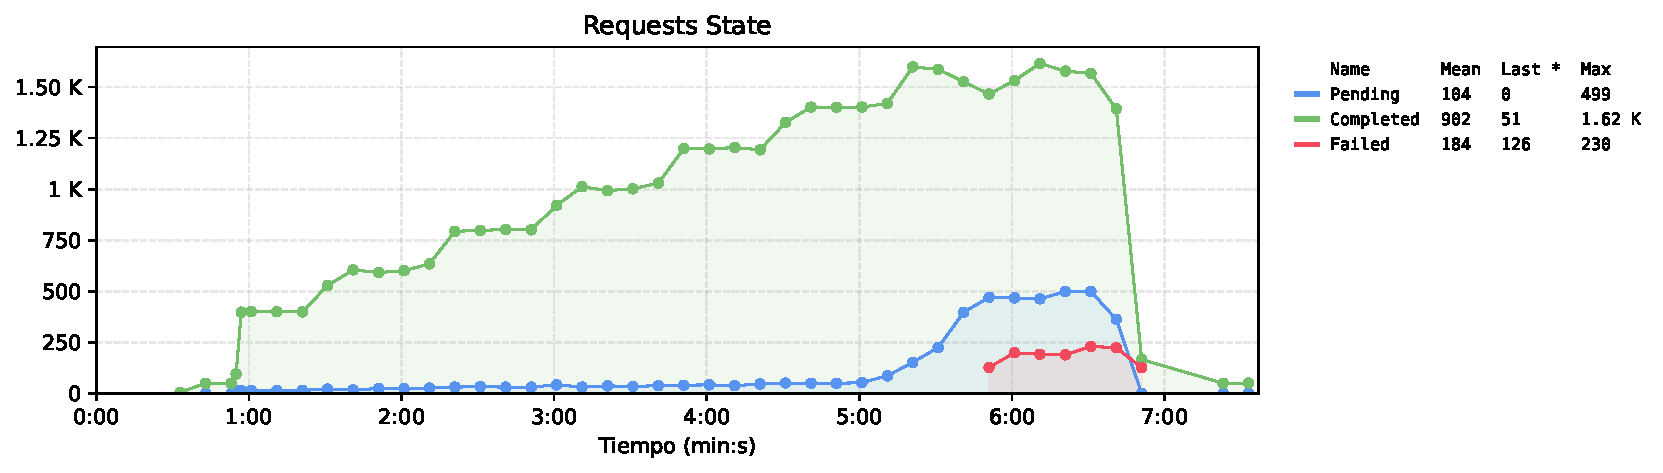
\includegraphics[width=0.5\columnwidth]{figures/propuesta_1/stress/requests_state}%
                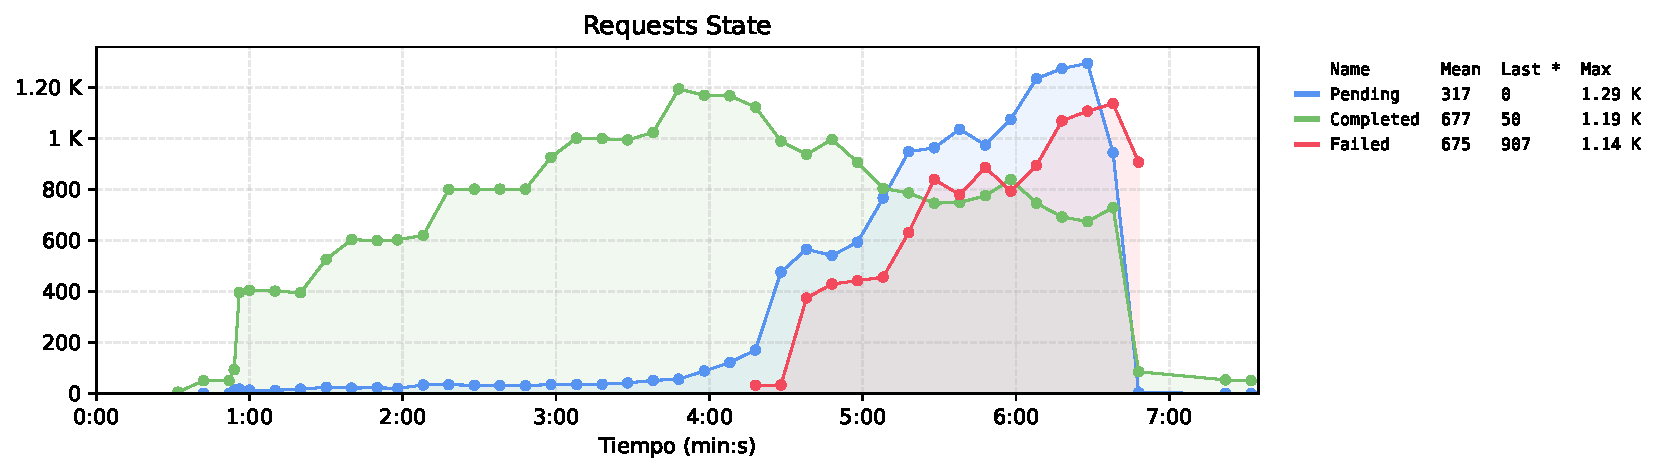
\includegraphics[width=0.5\columnwidth]{figures/sistema_base/stress/requests_state}
                \caption{
                    Comparativa de la disponibilidad ofrecida por la propuesta 1 (izquierda) y el sistema base (derecha) frente a un escenario de estrés.
                    La propuesta 1 obtuvo un incremento en el promedio de respuestas satisfactorias de 225 respuestas adicionales, lo que representa un aumento del $33,23\%$ frente al caso base.
                }
                \label{fig:comparacion_propuesta_1_sistema_base_stress_requests_state}
            \end{figure}

        \subsubsection{Latencia}
        \label{sec:propuesta_1_pruebas_de_stress_metricas_latencia}

            \begin{figure}[H]
                \centering
                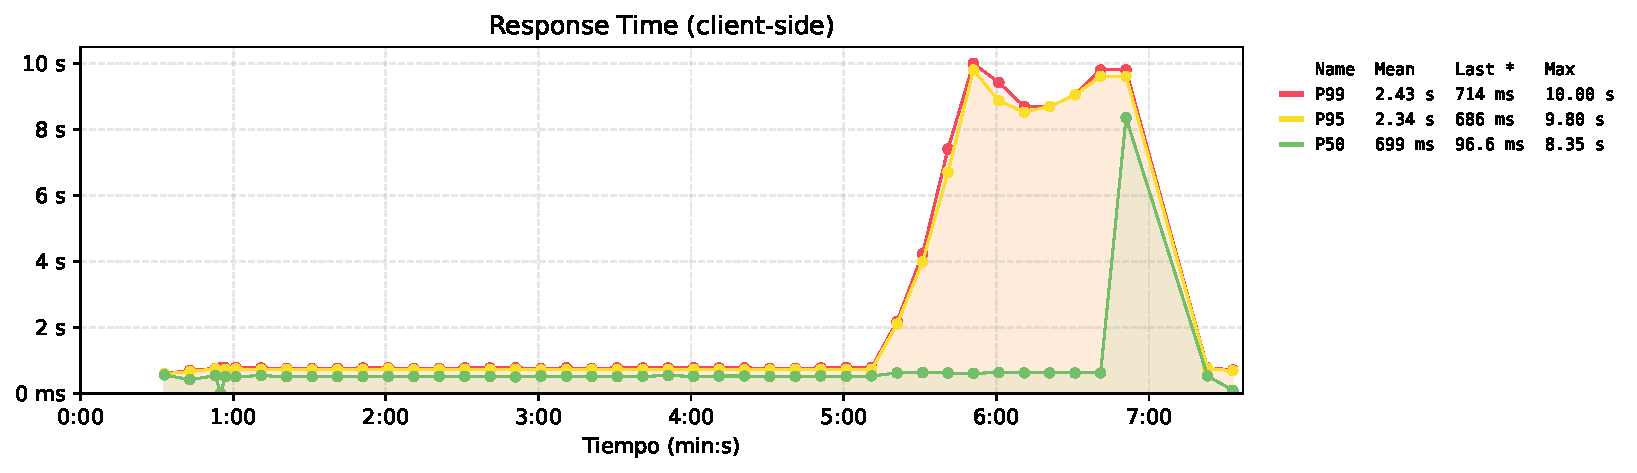
\includegraphics[width=0.5\columnwidth]{figures/propuesta_1/stress/response_time}%
                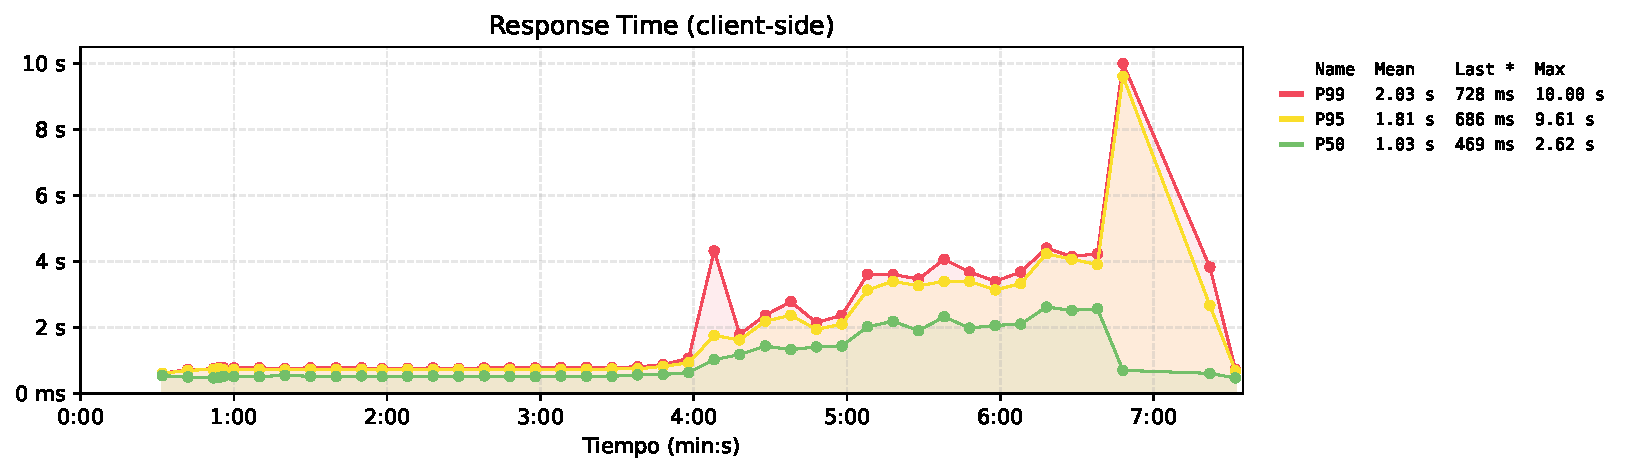
\includegraphics[width=0.5\columnwidth]{figures/sistema_base/stress/response_time}
                \caption{
                    Comparativa de los resultados de latencia entre la propuesta 1 (izquierda) y el sistema base (derecha) frente a un escenario de estrés.
                    Se observa que la propuesta 1 mejoro el promedio de latencia para P50.
                    Tambien se observa que empeoro en P95 y P99.
                }
                \label{fig:comparacion_propuesta_1_sistema_base_stress_response_time}
            \end{figure}

            \begin{figure}[H]
                \centering
                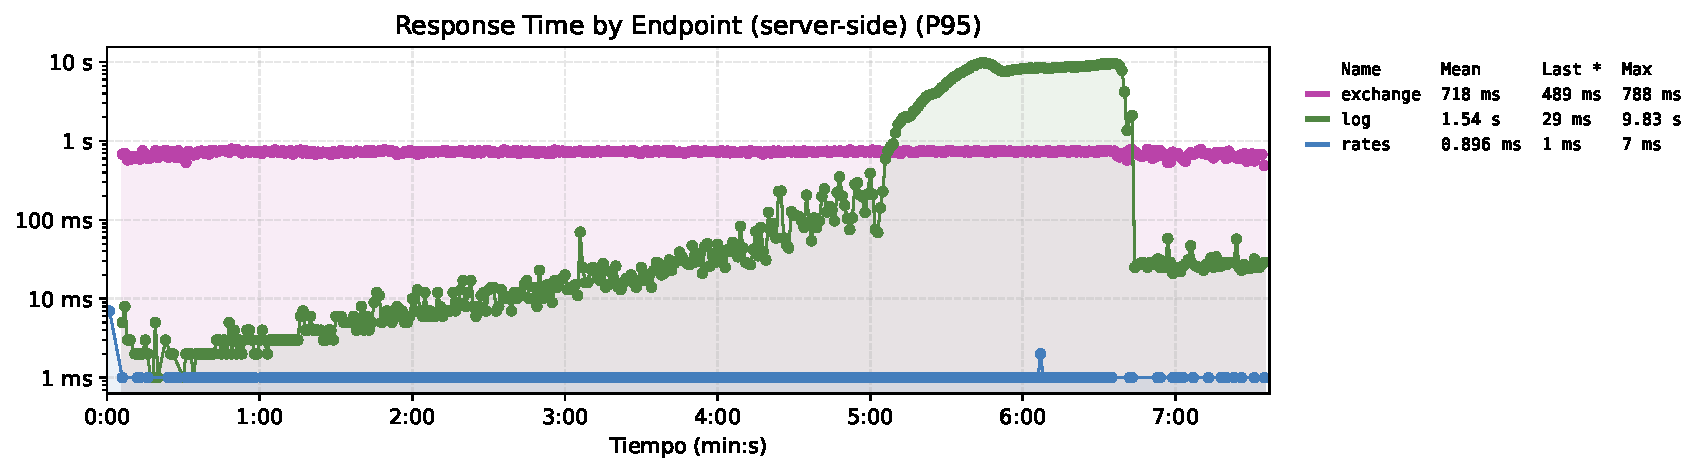
\includegraphics[width=0.5\columnwidth]{figures/propuesta_1/stress/endpoint_response_time}%
                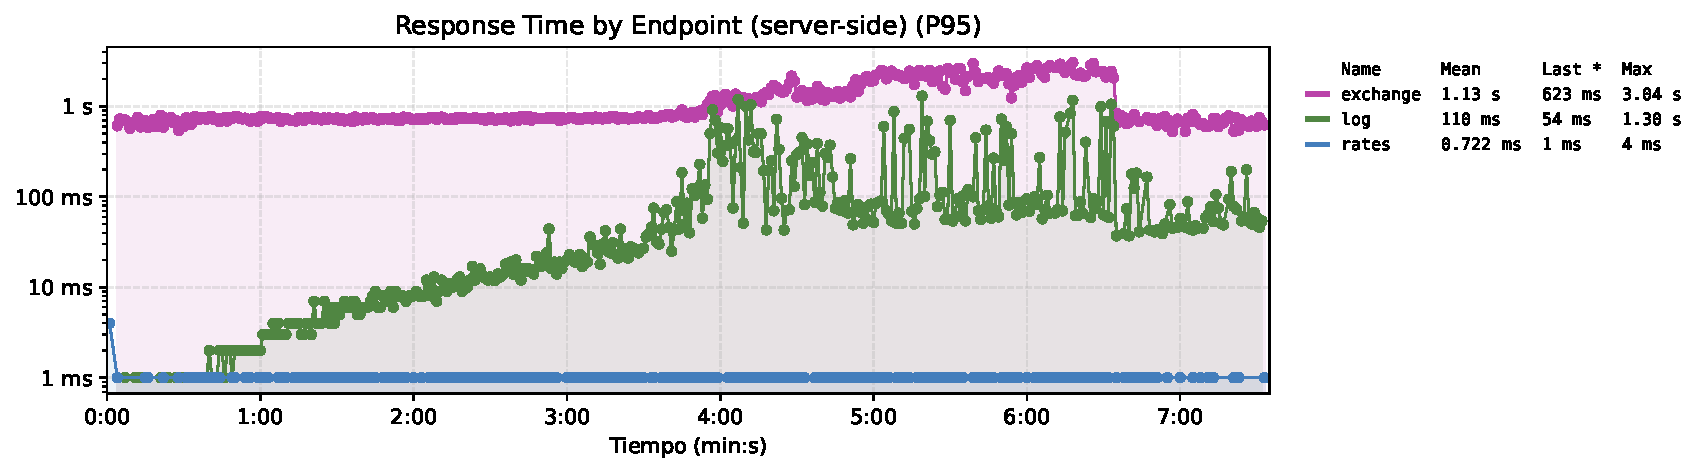
\includegraphics[width=0.5\columnwidth]{figures/sistema_base/stress/endpoint_response_time}
                \caption{
                    Comparativa de los resultados de latencia por endpoint entre la propuesta 1 (izquierda) y el sistema base (derecha) frente a un escenario de estrés.
                    Con diferencia el analisis mas interesante, la propuesta 1 permitio como se esperaba mejorar la latencia en el endpoint de exchange,
                    se puede notar que este no se ve afectado por la degradacion del endpoint de logs. Como si ocurria en el caso base, donde al rededor del minuto 4,
                    los tiempos de respuesta de exchange incrementaban, en este caso, los tiempos de respuesta se mantienen estables en 1 segundo, acotado por la dependencia
                    del servicio externo.
                    Por otro lado, los tiempos de respuesta de /log empeoraron, sinembargo es esperable, la mayor disponibilidad antes mencionada implica que se
                    registraron mas transacciones, por lo que el tamaño del log necesariamente aumento.
                    Esto explica el aumento de los tiempos de respuesta visto desde el lado del cliente antes mencionados, sinembargo, las metricas se ven ensuciadas
                    al mezclar todos los endpoints.
                }
                \label{fig:comparacion_propuesta_1_sistema_base_stress_endpoint_response_time}
            \end{figure}

        \subsubsection{Uso de recursos}
        \label{sec:propuesta_1_pruebas_de_stress_metricas_recursos}

            \begin{figure}[H]
                \centering
                \begin{minipage}[c]{0.5\columnwidth}
                    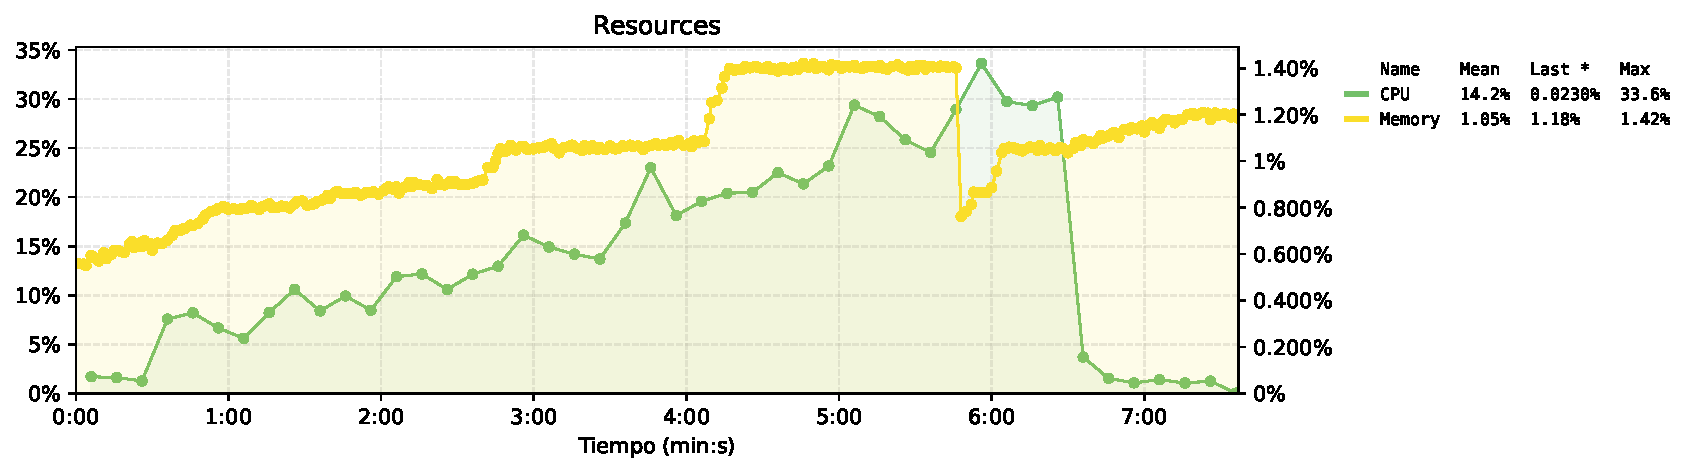
\includegraphics[width=\linewidth]{figures/propuesta_1/stress/resources}\\
                    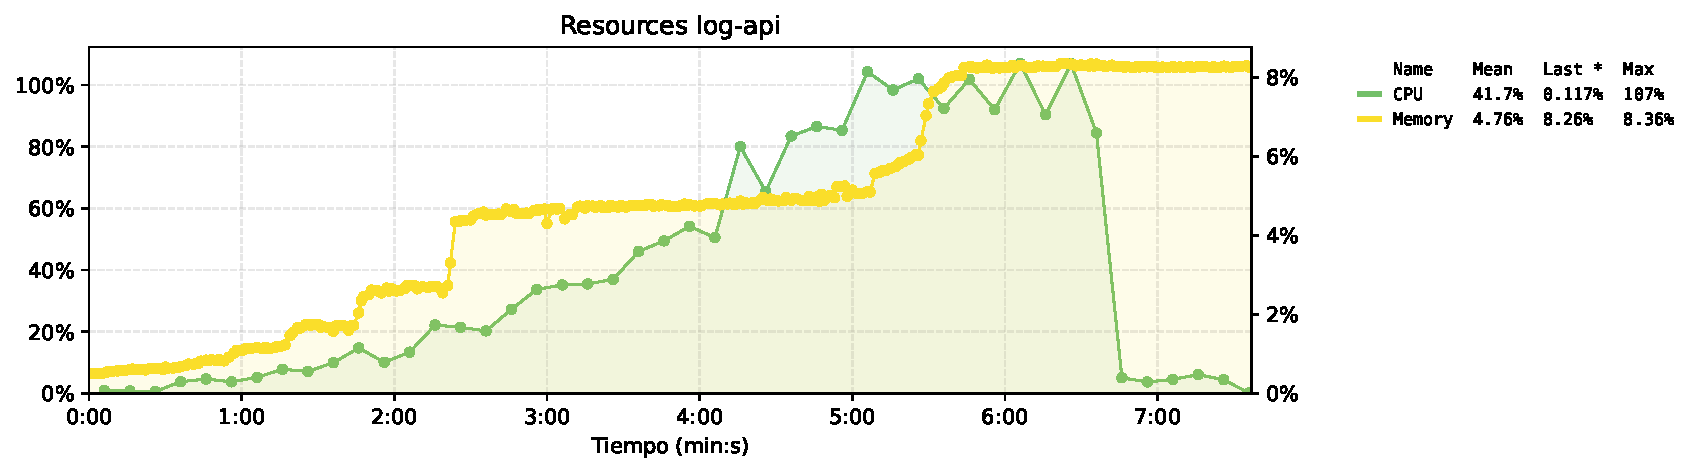
\includegraphics[width=\linewidth]{figures/propuesta_1/stress/resources_log_api}
                \end{minipage}%
                \begin{minipage}[c]{0.5\columnwidth}
                    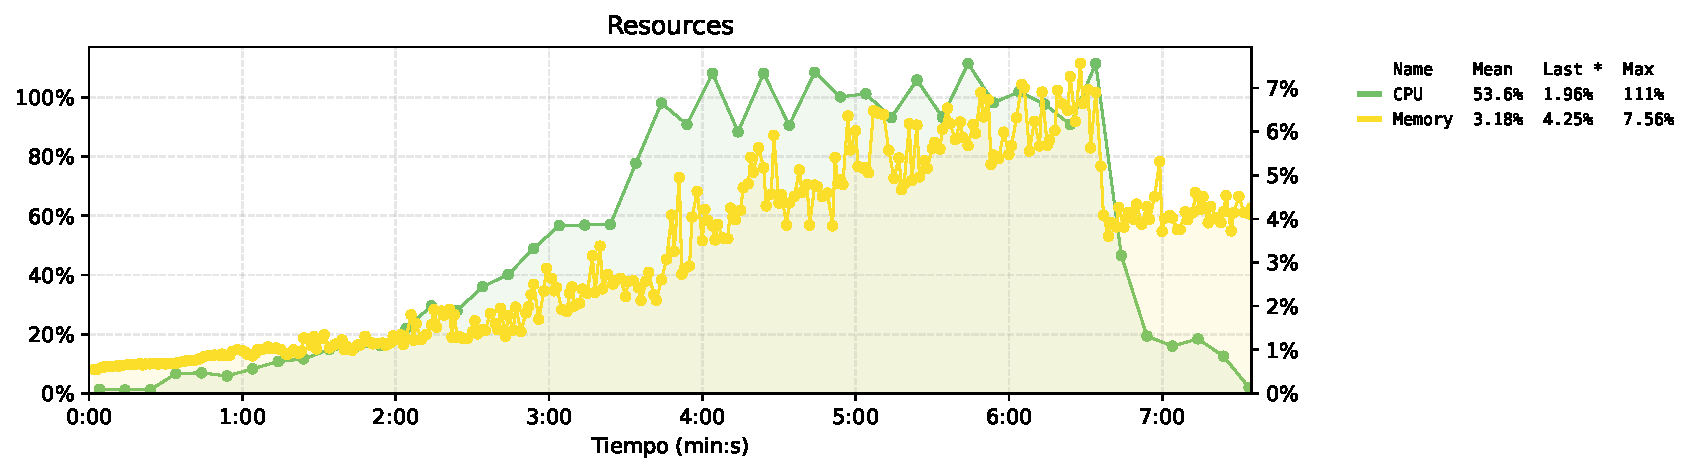
\includegraphics[width=\linewidth]{figures/sistema_base/stress/resources}
                \end{minipage}
                \caption{
                    Comparativa de los resultados del uso de recursos entre la propuesta 1 (izquierda) y el sistema base (derecha) frente a un escenario de estrés.
                    Destacar que consideramos la comparacion con respecto a ambos nodos, el nodo de exchange y el de logs.
                    Se puede observar que el nodo de logs mantiene la carga con respecto a la del sistema base, incluso la aumenta.
                    Esto es esperable con el aumento de la disponibilidad, mas request completadas implican mas entradas en el log.
                    Sinembargo, el nodo de exchange apenas llego a un $14.2\%$ de uso de CPU y $1.42\%$ de uso de memoria.
                }
                \label{fig:comparacion_propuesta_1_sistema_base_stress_resources}
            \end{figure}

        \subsubsection{Volumen operado por moneda}
        \label{sec:propuesta_1_pruebas_de_stress_metricas_volumen_operado_por_moneda}

            \begin{figure}[H]
                \centering
                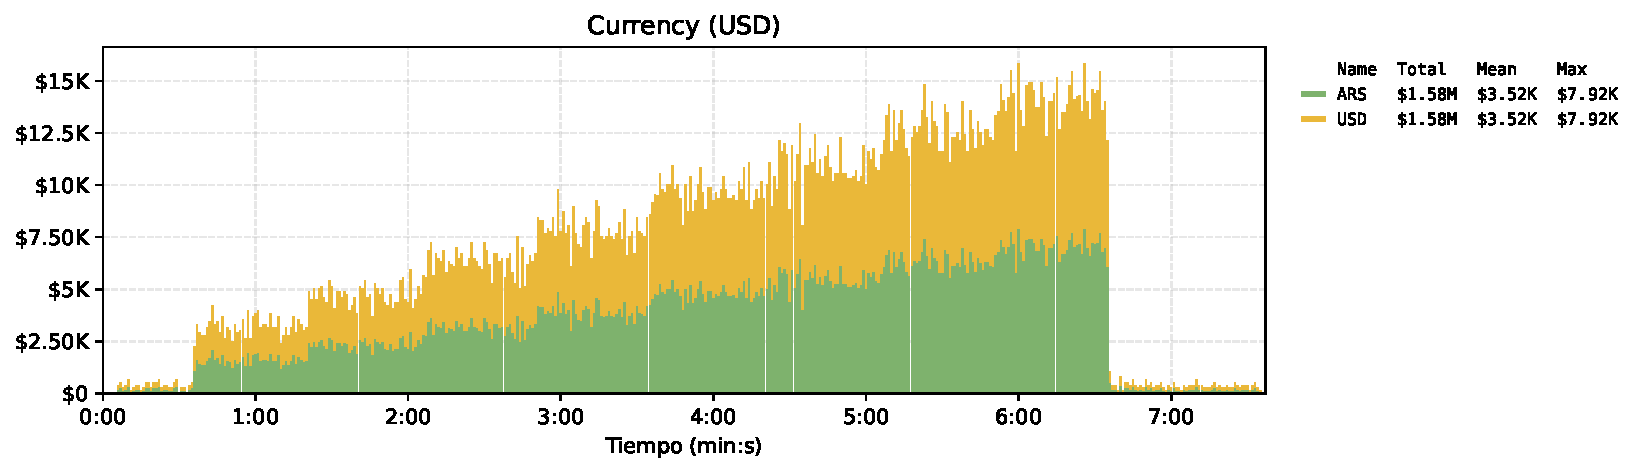
\includegraphics[width=0.5\columnwidth]{figures/propuesta_1/stress/currency}%
                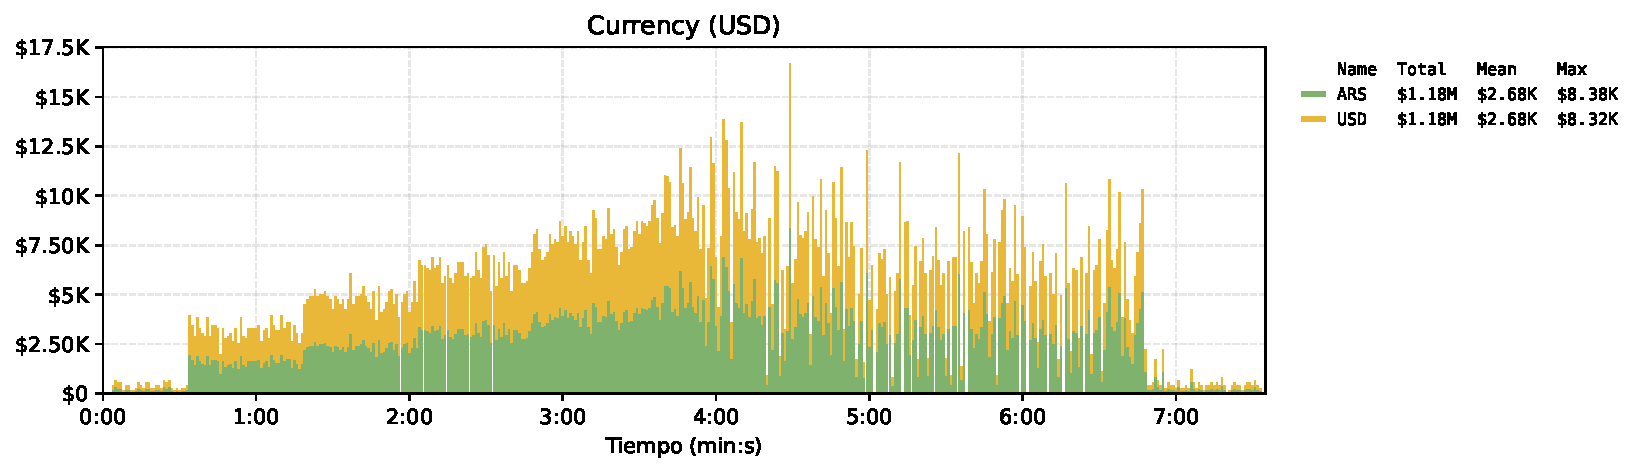
\includegraphics[width=0.5\columnwidth]{figures/sistema_base/stress/currency}
                \caption{
                    Comparativa de los resultados de volumen operado en cada moneda entre la propuesta 1 (izquierda) y el sistema base (derecha) frente a un escenario de estrés.
                    Se observa que la propuesta 1 obtuvo un mayor volumen total siendo este $1.58M$ frente al $1.18M$ del sistema base, es decir una mejora del $33.90\%$.
                }
                \label{fig:comparacion_propuesta_1_sistema_base_stress_currency}
            \end{figure}

        \subsubsection{Volumen neto operado}
        \label{sec:propuesta_1_pruebas_de_stress_metricas_volumen_neto_operado_por_moneda}

            \begin{figure}[H]
                \centering
                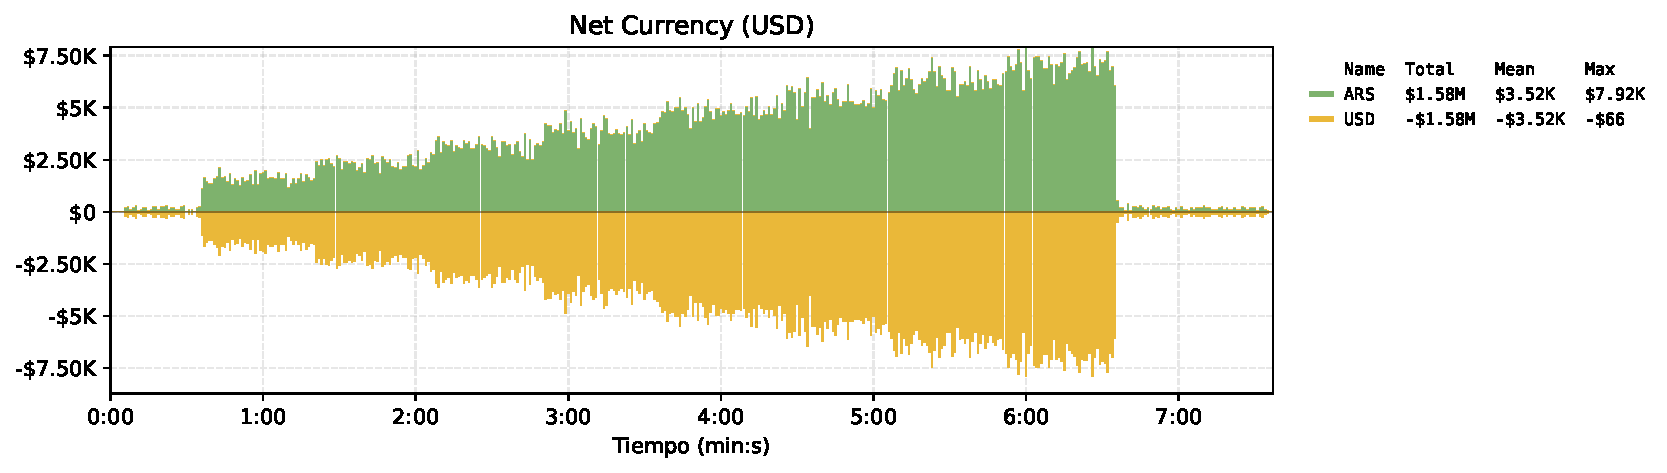
\includegraphics[width=0.5\columnwidth]{figures/propuesta_1/stress/net_currency}%
                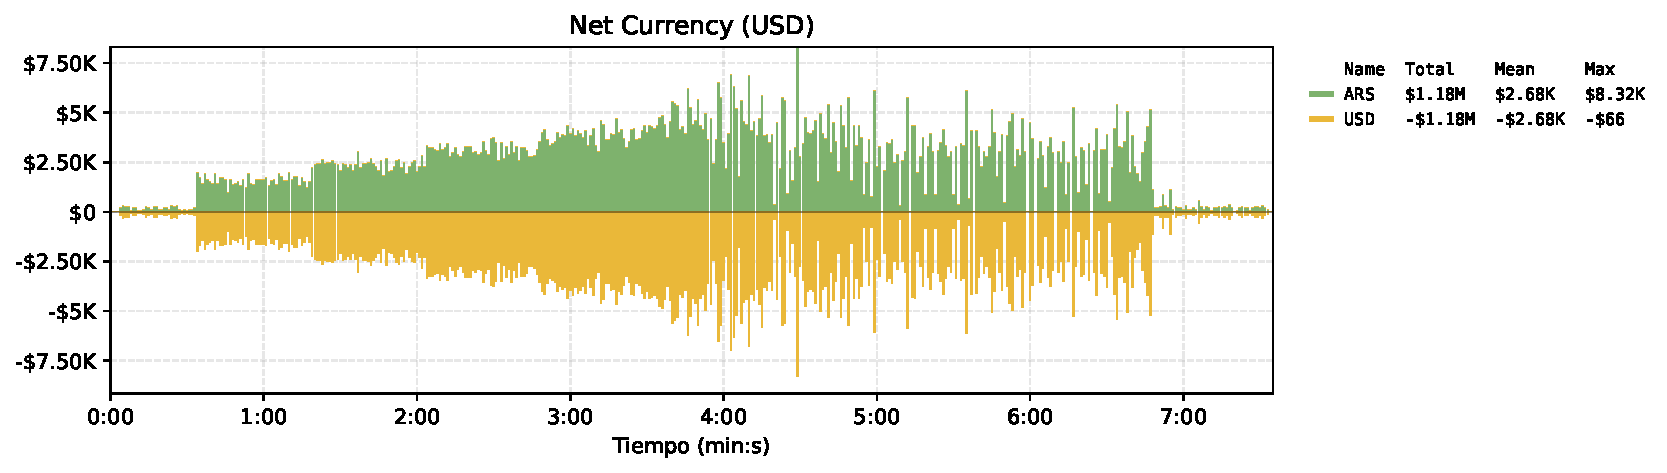
\includegraphics[width=0.5\columnwidth]{figures/sistema_base/stress/net_currency}
                \caption{
                    Comparativa de los resultados de volumen neto operado en cada moneda entre la propuesta 1 (izquierda) y el sistema base (derecha) frente a un escenario de estrés.
                    Analogamente al volumen operado, se observa que el volumen neto tambien es mayor en la propuesta 1 frente al sistema base.
                }
                \label{fig:comparacion_propuesta_1_sistema_base_stress_net_currency}
            \end{figure}

    \subsection{Pruebas de resistencia}
    \label{sec:propuesta_1_pruebas_de_soak}

    La prueba de resistencia se realizo usando una tasa constante de 40 usuarios durante 2700s (45 minutos).
    Se realizo un warm-up inicial de 5 usuarios durante 60s. Ademas, al final de la prueba se dejo una instancia de recovery de nuevamente 5 usuarios esta vez durante 120s (2 minutos).
    Tampoco se realizaron recargas de saldo intermedias y se mantuvo el mismo uso de endpoints para que los resultados sean comparables.

        \subsubsection{Disponibilidad}
        \label{sec:propuesta_1_pruebas_de_soak_metricas_disponibilidad}

            \begin{figure}[H]
                \centering
                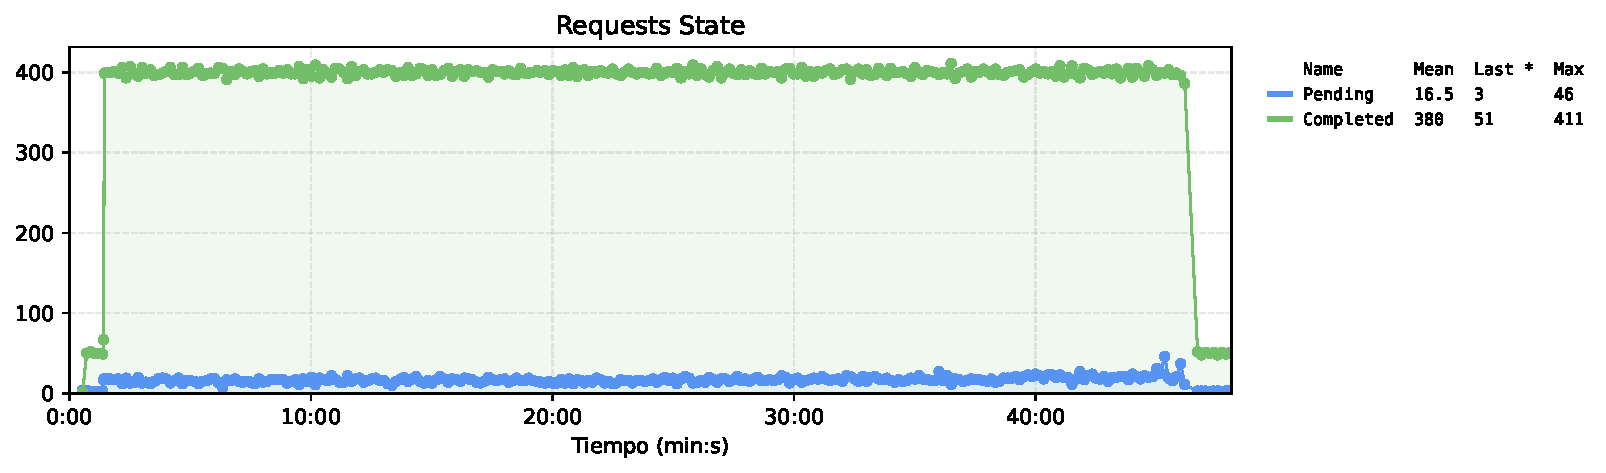
\includegraphics[width=0.5\columnwidth]{figures/propuesta_1/soak/requests_state}%
                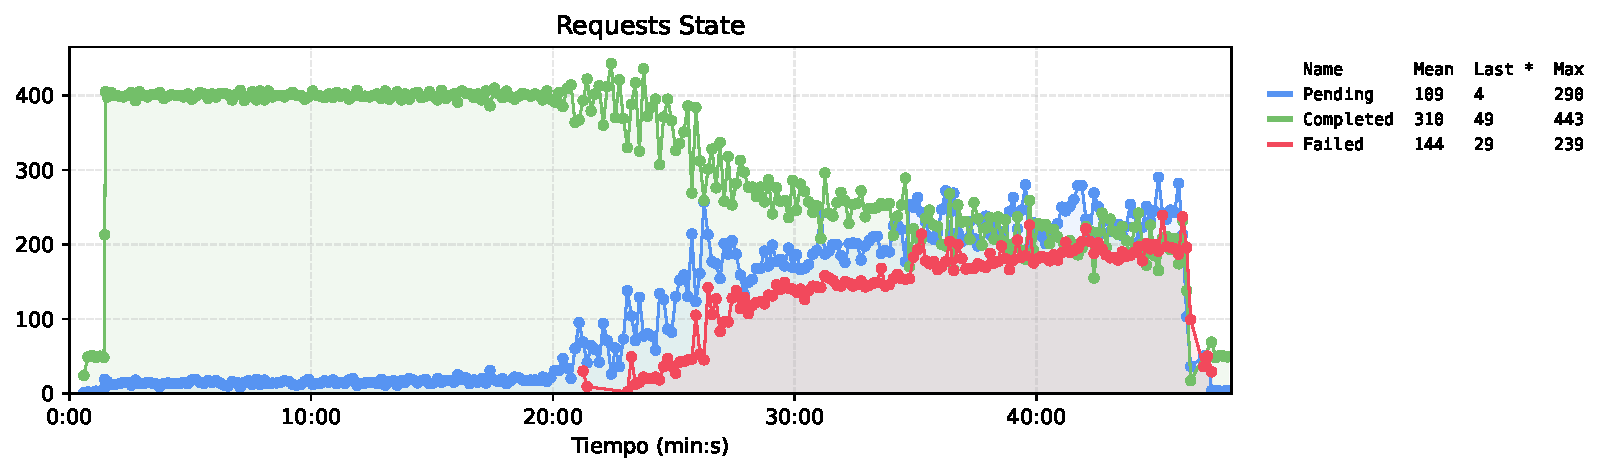
\includegraphics[width=0.5\columnwidth]{figures/sistema_base/soak/requests_state}
                \caption{
                    Comparativa de la disponibilidad ofrecida por la propuesta 1 (izquierda) y el sistema base (derecha) frente a un scenario de resistencia.
                    El sistema base mostraba una degradacion critica a los 20 minutos, mientras que la propuesta 1 logro completar satisfactoriamente todas las request durante los 45 minutos.
                }
                \label{fig:comparacion_propuesta_1_sistema_base_soak_requests_state}
            \end{figure}

        \subsubsection{Latencia}
        \label{sec:propuesta_1_pruebas_de_soak_metricas_latencia}

            \begin{figure}[H]
                \centering
                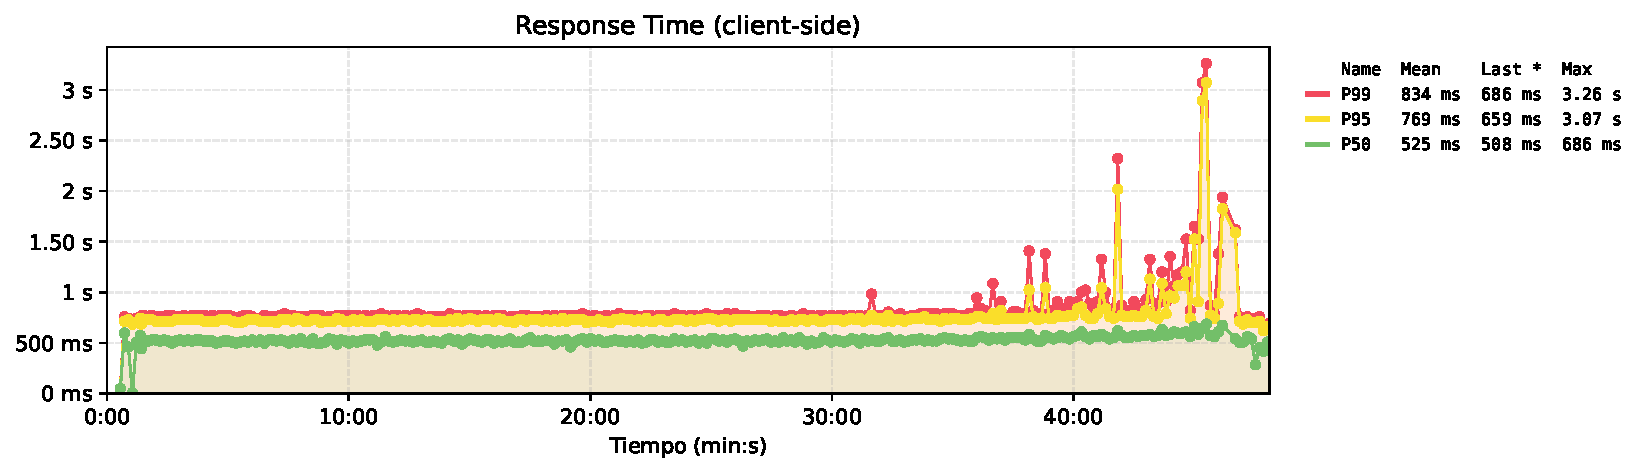
\includegraphics[width=0.5\columnwidth]{figures/propuesta_1/soak/response_time}%
                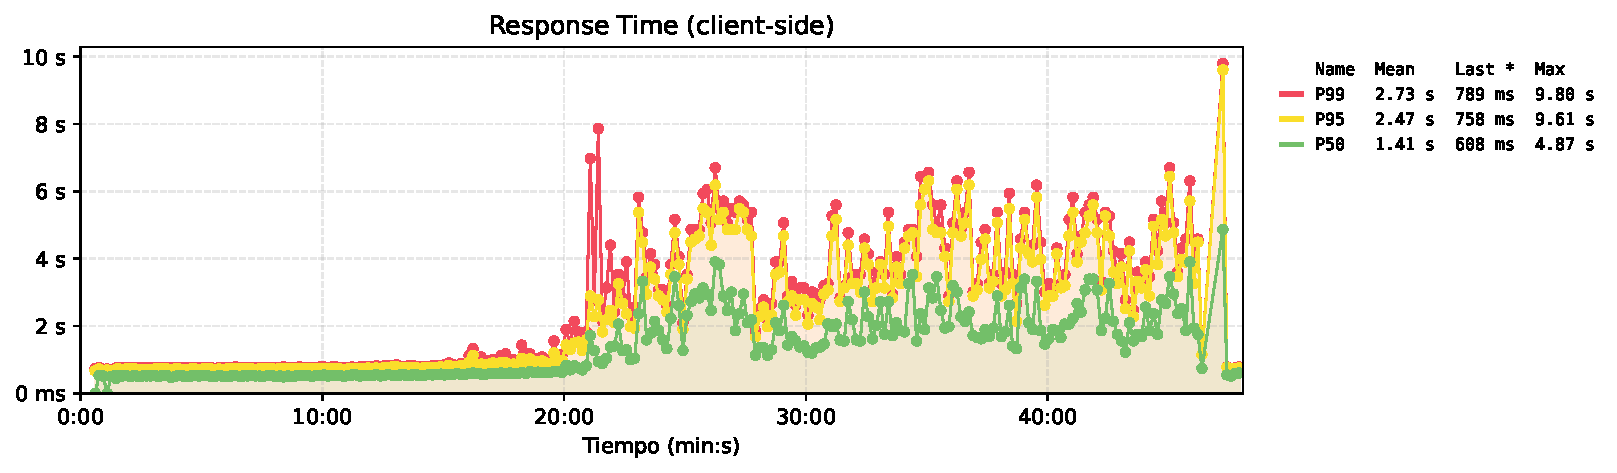
\includegraphics[width=0.5\columnwidth]{figures/sistema_base/soak/response_time}
                \caption{
                    Comparativa de los resultados de latencia entre la propuesta 1 (izquierda) y el sistema base (derecha) frente a un scenario de resistencia.
                    Consistente con los resultados de disponibilidad se muestra una gran mejora especialmente posterior al minuto 20. Sinembargo, la propuesta 1 sigue mostrando una principio de degradacion a los 40 minutos, esperable dado el crecimiento del log.
                }
                \label{fig:comparacion_propuesta_1_sistema_base_soak_response_time}
            \end{figure}

            \begin{figure}[H]
                \centering
                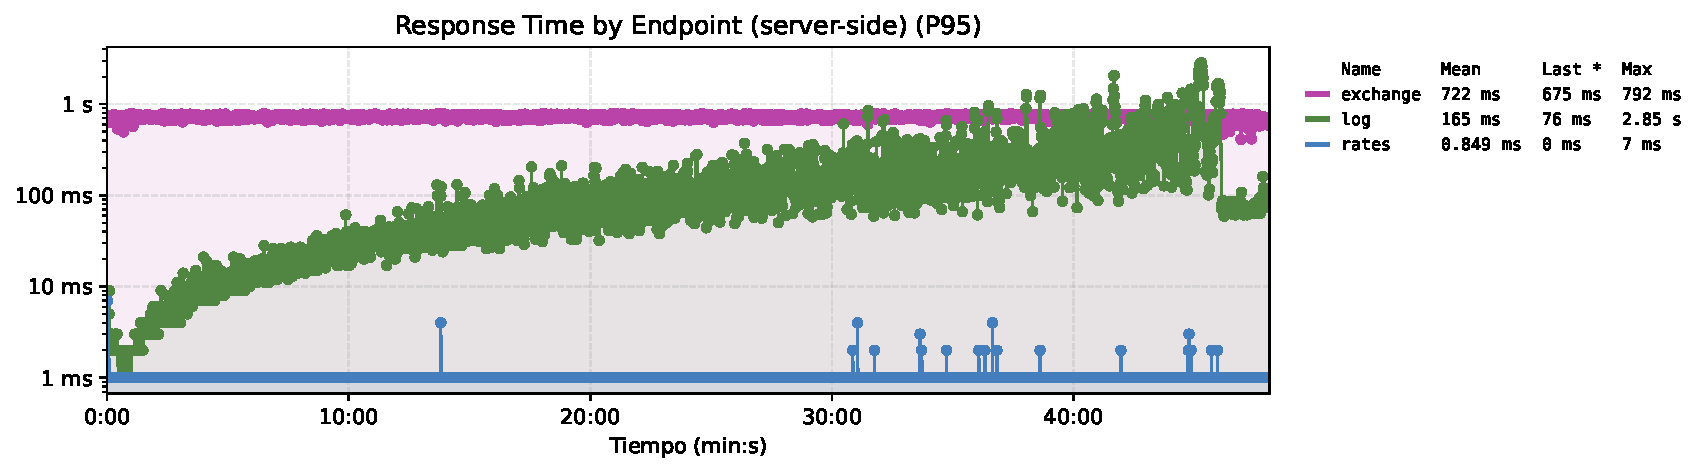
\includegraphics[width=0.5\columnwidth]{figures/propuesta_1/soak/endpoint_response_time}%
                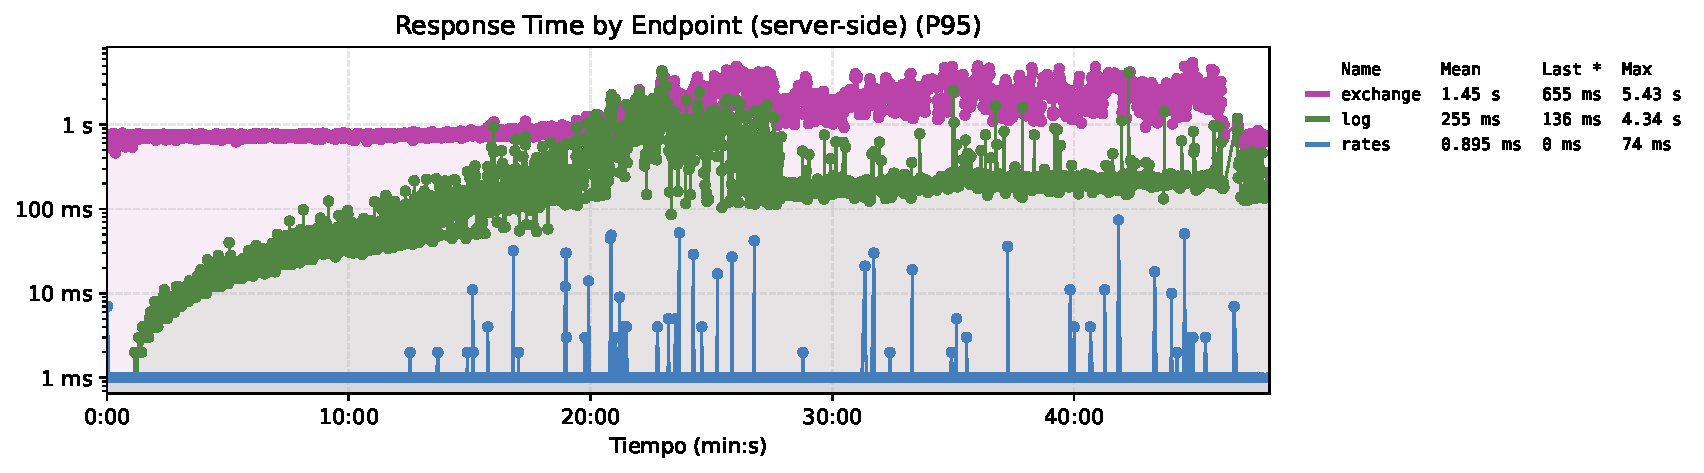
\includegraphics[width=0.5\columnwidth]{figures/sistema_base/soak/endpoint_response_time}
                \caption{
                    Comparativa de los resultados de latencia por endpoint entre la propuesta 1 (izquierda) y el sistema base (derecha) frente a un scenario de resistencia.
                    Para el tiempo de respuesta desde la perspectiva del servidor, se muestra como en la propuesta 1 los tiempos del endpoint de logs ya no “empujan” los tiempos del endpoint exchange, sinembargo como ya se menciono, el endpoint de logs continua degradando.
                    Los tiempos de respuesta de log entre ambos casos lamentablemente no son comparables puesto que menor disponibilidad implica un menor crecimiento del propio log.
                }
                \label{fig:comparacion_propuesta_1_sistema_base_soak_endpoint_response_time}
            \end{figure}

        \subsubsection{Uso de recursos}
        \label{sec:propuesta_1_pruebas_de_soak_metricas_recursos}

            \begin{figure}[H]
                \centering
                \begin{minipage}[c]{0.5\columnwidth}
                    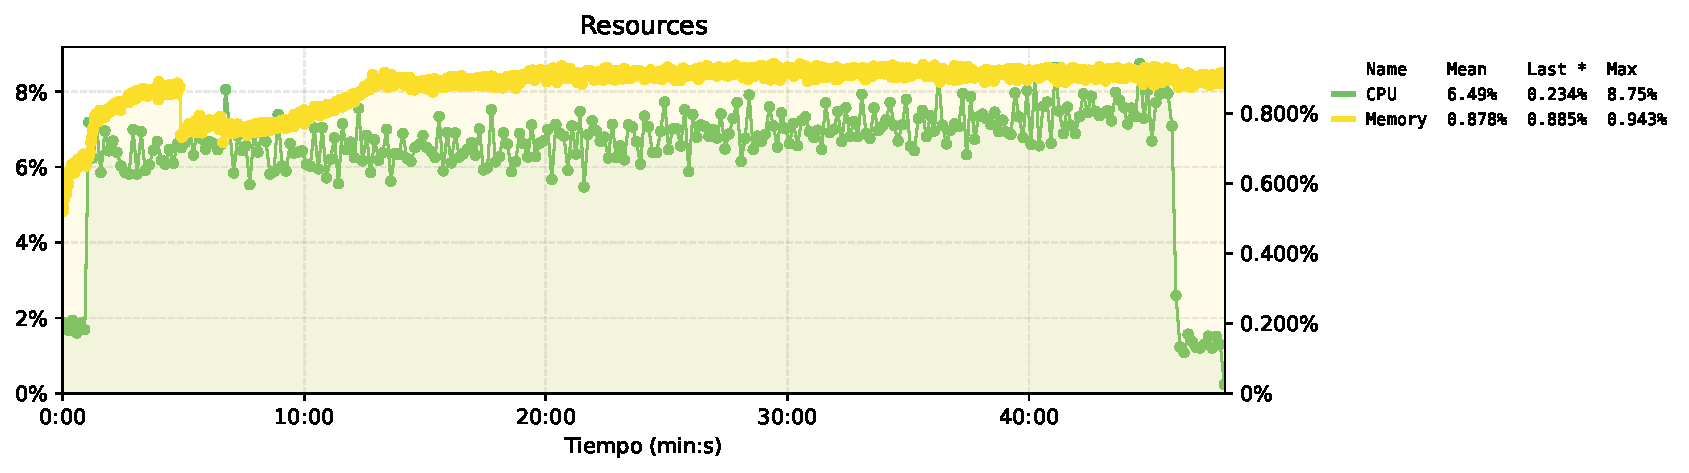
\includegraphics[width=\linewidth]{figures/propuesta_1/soak/resources}\\
                    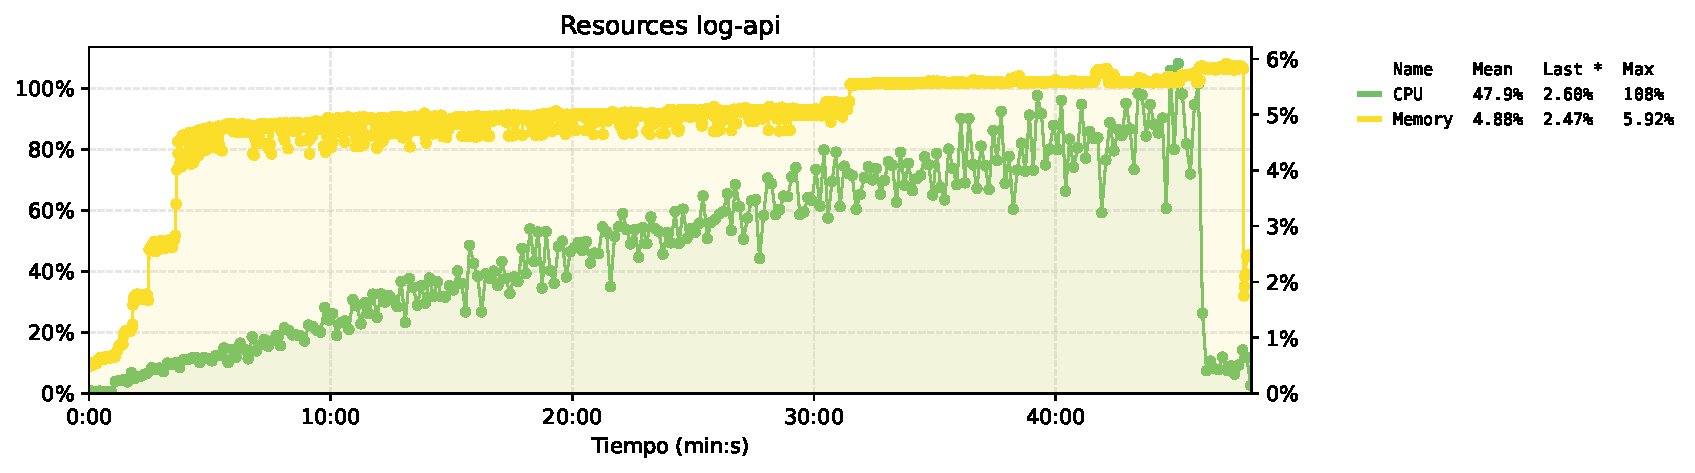
\includegraphics[width=\linewidth]{figures/propuesta_1/soak/resources_log_api}
                \end{minipage}%
                \begin{minipage}[c]{0.5\columnwidth}
                    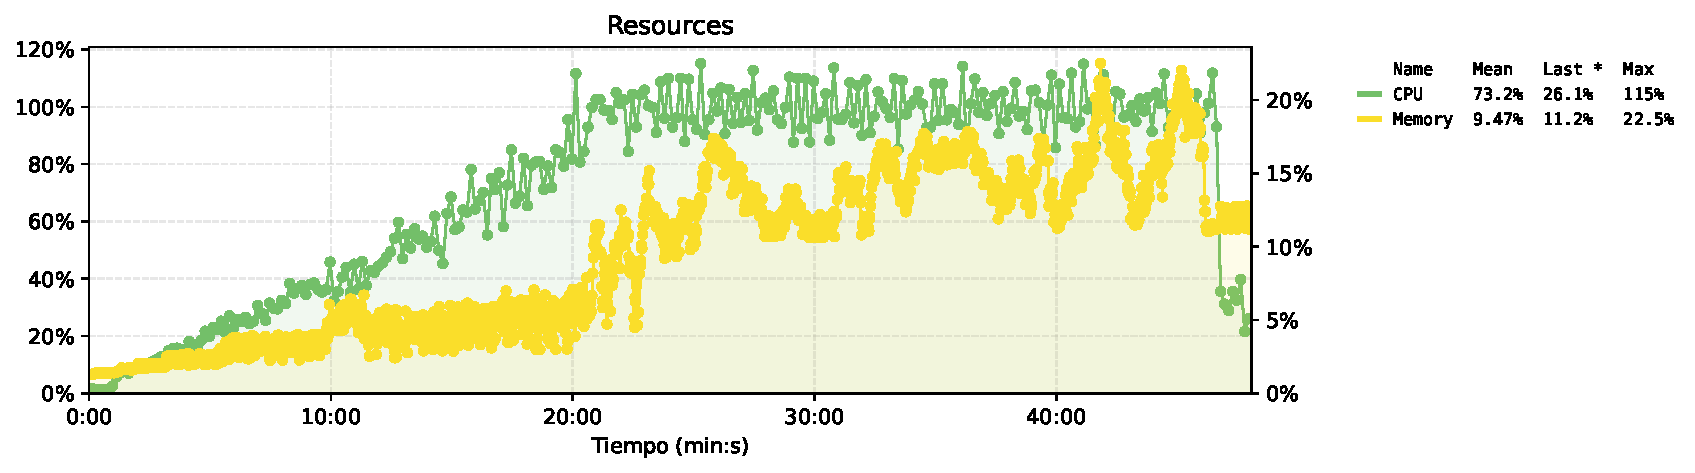
\includegraphics[width=\linewidth]{figures/sistema_base/soak/resources}
                \end{minipage}
                \caption{
                    Comparativa de los resultados del uso de recursos entre la propuesta 1 (izquierda) y el sistema base (derecha) frente a un scenario de resistencia.
                    Destacar que ambos casos no son directamente comparables, la propuesta 1 dispone de dos contenedores/nodos independientes cada uno con los mismo recursos que el nodo monolitico del escenario base.
                    Se observa que para el nodo de exchange-api los recursos son practicamente ociosos con apenas un uso del $6.4\%$ de CPU y $0.8\%$ en memoria. Tambien se observa en los recursos del nodo de logs, un uso mas constante de la memoria, esperable al stremear los datos desde disco y no conservar todos los logs en memoria.
                }
                \label{fig:comparacion_propuesta_1_sistema_base_soak_resources}
            \end{figure}

        \subsubsection{Volumen operado por moneda}
        \label{sec:propuesta_1_pruebas_de_soak_metricas_volumen_operado_por_moneda}

            \begin{figure}[H]
                \centering
                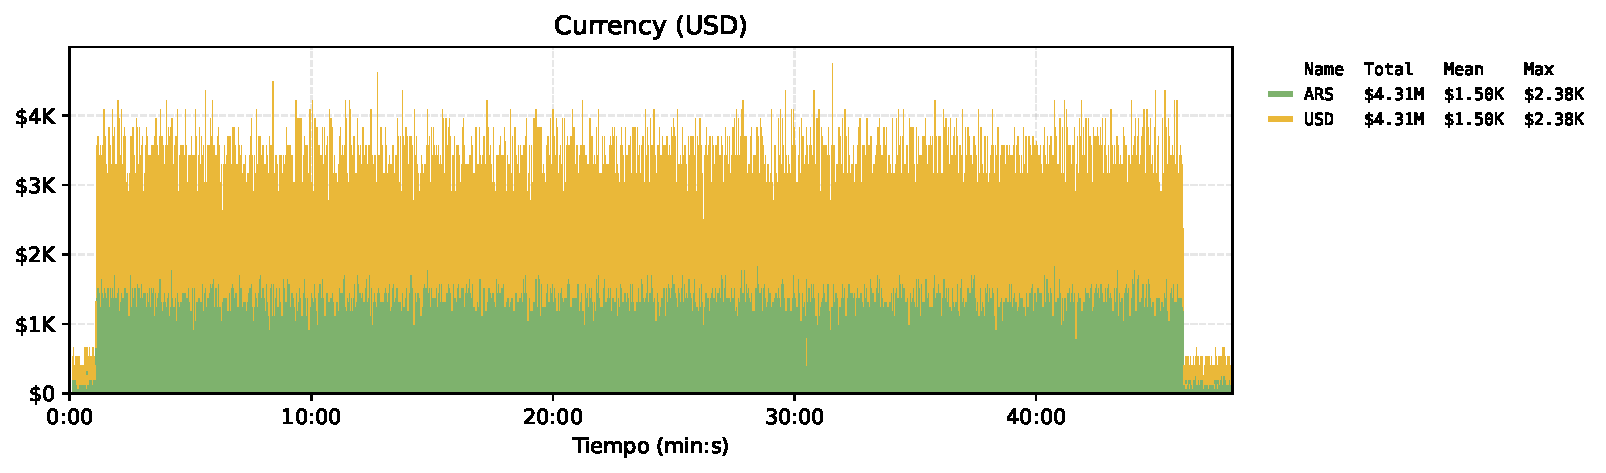
\includegraphics[width=0.5\columnwidth]{figures/propuesta_1/soak/currency}%
                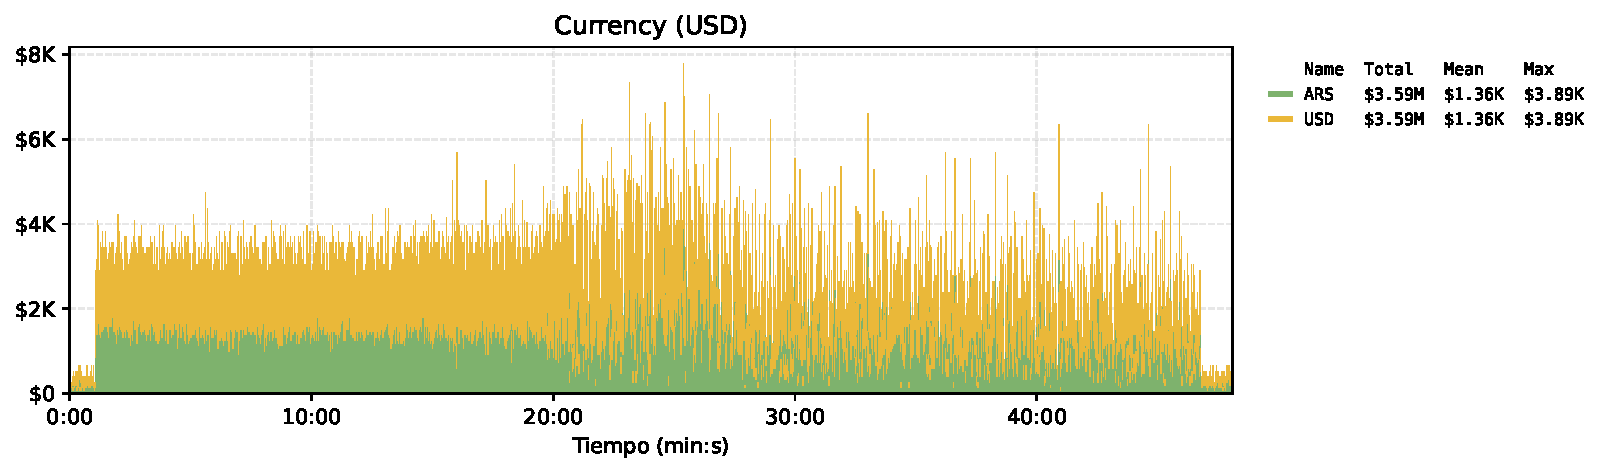
\includegraphics[width=0.5\columnwidth]{figures/sistema_base/soak/currency}
                \caption{
                    Comparativa de los resultados de volumen operado en cada moneda entre la propuesta 1 (izquierda) y el sistema base (derecha) frente a un scenario de resistencia.
                    Se observa que la propuesta 1 obtuvo un mayor volumen total siendo este $4.31M$ frente al $3.59M$ del sistema base, es decir una mejora del $20.06\%$.
                }
                \label{fig:comparacion_propuesta_1_sistema_base_soak_currency}
            \end{figure}

        \subsubsection{Volumen neto operado}
        \label{sec:propuesta_1_pruebas_de_soak_metricas_volumen_neto_operado_por_moneda}

            \begin{figure}[H]
                \centering
                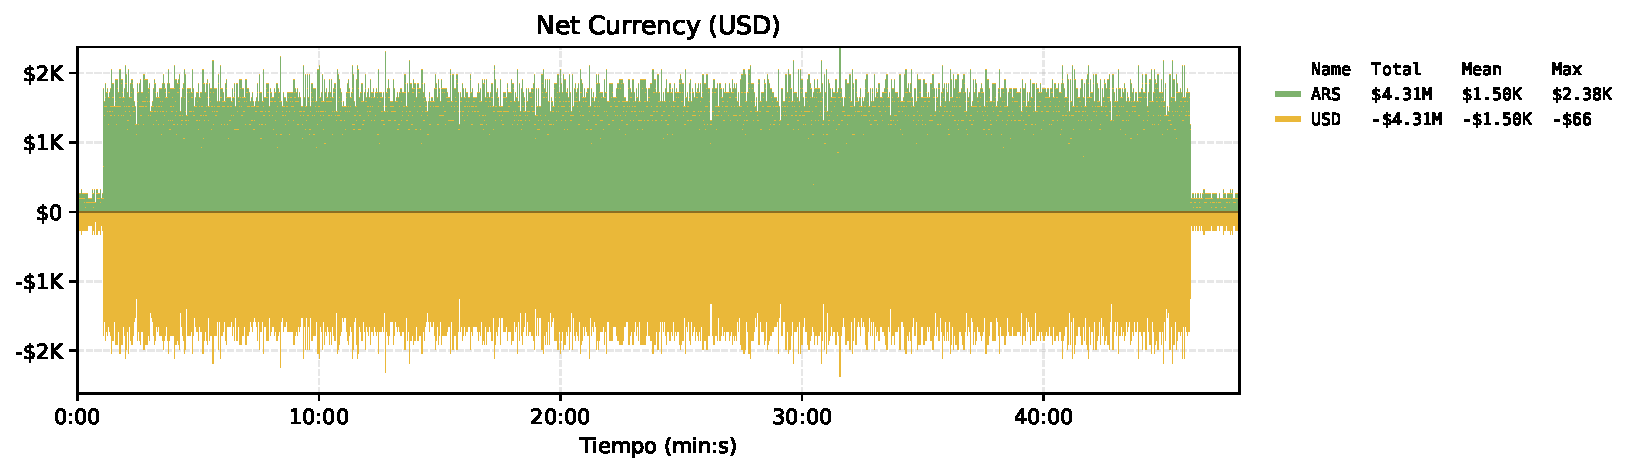
\includegraphics[width=0.5\columnwidth]{figures/propuesta_1/soak/net_currency}%
                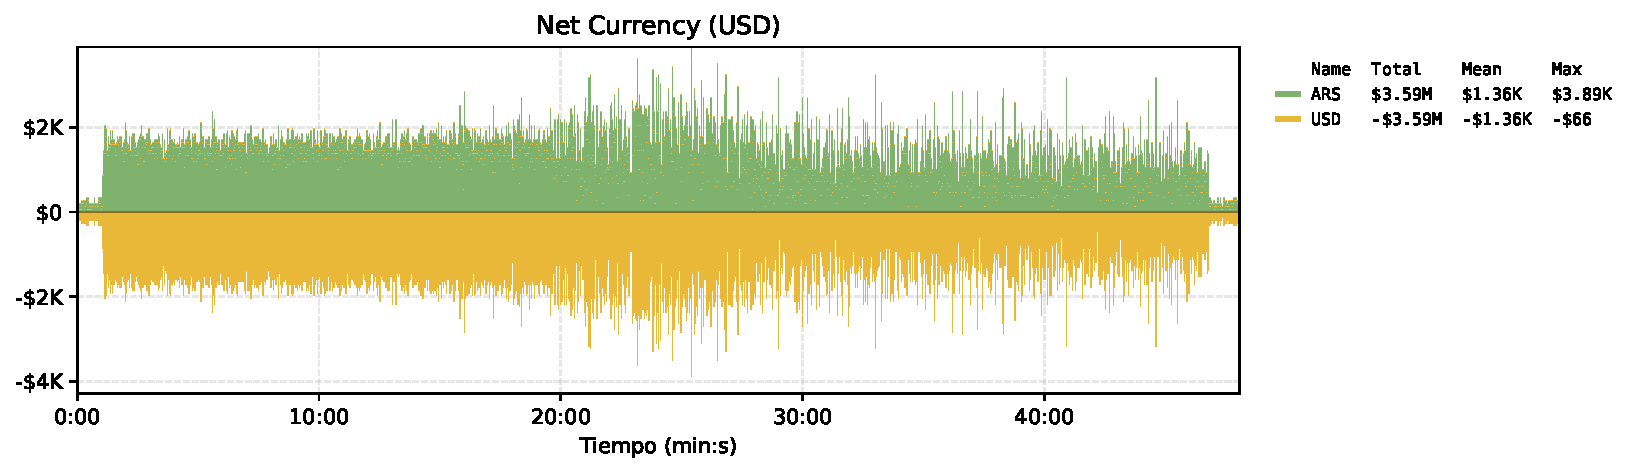
\includegraphics[width=0.5\columnwidth]{figures/sistema_base/soak/net_currency}
                \caption{
                    Comparativa de los resultados de volumen neto operado en cada moneda entre la propuesta 1 (izquierda) y el sistema base (derecha) frente a un scenario de resistencia.
                    Analogamente al volumen operado, se observa que el volumen neto tambien es mayor en la propuesta 1 frente al sistema base en la misma proporcion.
                }
                \label{fig:comparacion_propuesta_1_sistema_base_soak_net_currency}
            \end{figure}

    \subsection{Resultados y conclusiones}
    \label{sec:propuesta_1_resultados_y_conclusiones}

    La propuesta 1 demostro ser capaz de aislar la degradacion producida por la consulta de logs de las opeeraciones de negocio del sistema, permitiendo ofrecer una mejor disponibilidad a los usuarios comunes.
    Por otro lado la consulta de logs sigue degradandose con el tiempo. Sinembargo, este desacoplamiento propuesto permitiria replicar el nodo de consulta para dar soporte de lectura de los a mas usuarios, es decir, permitiendo escalabilidad horizontal.
